\documentclass[11pt,a4paper]{article}

\usepackage[margin=22mm,headheight=14pt]{geometry}

\usepackage{longtable,booktabs,array,hyperref,xcolor,tikz,fancyhdr}

\usepackage{fontspec,xeCJK}

\setmainfont[Ligatures=TeXOff]{Times New Roman}

\setsansfont[Ligatures=TeXOff]{Times New Roman}

\setmonofont[Ligatures=TeXOff,WordSpace={1,1,1}]{Times New Roman}

\setCJKmainfont{Noto Serif CJK SC}

\setCJKsansfont{Noto Serif CJK SC}

\setCJKmonofont{Noto Serif CJK SC}

\newfontfamily\vulcanmathsymbols{Noto Serif CJK SC}

\XeTeXgenerateactualtext=1

\definecolor{vulcan}{HTML}{BB3E23}

\pgfdeclarelayer{connections}\pgfdeclarelayer{edge labels}\pgfsetlayers{connections,main,edge labels}

\hypersetup{hidelinks}

\newcolumntype{L}[1]{>{\raggedright\arraybackslash}p{#1}}

\setlength{\emergencystretch}{5em}\tolerance=2000\hbadness=10000

\setlength{\parindent}{0pt}\setlength{\parskip}{5pt}

\pagestyle{fancy}\fancyhf{}\fancyhead[L]{\small\sffamily VULCAN}

\fancyhead[R]{\small Product design and verification}\fancyfoot[C]{\thepage}

\begin{document}

{\sffamily\huge\raggedright\textbf{RIVET-A2: AES-128/\allowbreak{}256 and Authenticated AES-GCM RTL IP}\par}

{\large Technical Design and Verification Report}\par

16 October 2026 (\allowbreak{}UTC+\allowbreak{}8)\allowbreak{}\par\textcolor{vulcan}{\rule{\textwidth}{0.5pt}}

\begin{abstract}

RIVET-A2 is a modular SystemVerilog cryptographic engine for raw AES-128/\allowbreak{}256 encryption and decryption and AES-GCM authenticated encryption and decryption. It preserves the RIVET-A1 iterative-round architecture while adding AES-256 key expansion,\allowbreak{} streamed additional authenticated data,\allowbreak{} partial payload blocks,\allowbreak{} full-width tags and authenticated-release storage.


Independent reference-based simulation passed at payload capacities of 1,\allowbreak{} 3,\allowbreak{} 16 and 256 blocks. All six targeted functional mutants were rejected,\allowbreak{} and generic Yosys synthesis passed at capacities 1,\allowbreak{} 3 and 16 with no inferred latches or unresolved modules. These results establish bounded functional and generic synthesis verification of RTL IP,\allowbreak{} not physical implementation or cryptographic certification.


\end{abstract}

\section{Architecture and design rationale}

The top-level controller admits one operation at a time and shares a single iterative AES engine between raw-block and GCM processing. A separate serial GHASH multiplier authenticates ordered AAD and ciphertext blocks. Both GCM directions buffer their entire payload until tag processing completes; payload release additionally requires consumption of the successful tag record. This sacrifices streaming output and overlap for a simple,\allowbreak{} externally testable authentication boundary. The following blocks are arranged row-major in three columns. Architecture and implementation are documented in E001 and embodied in E003–E011.

\begin{center}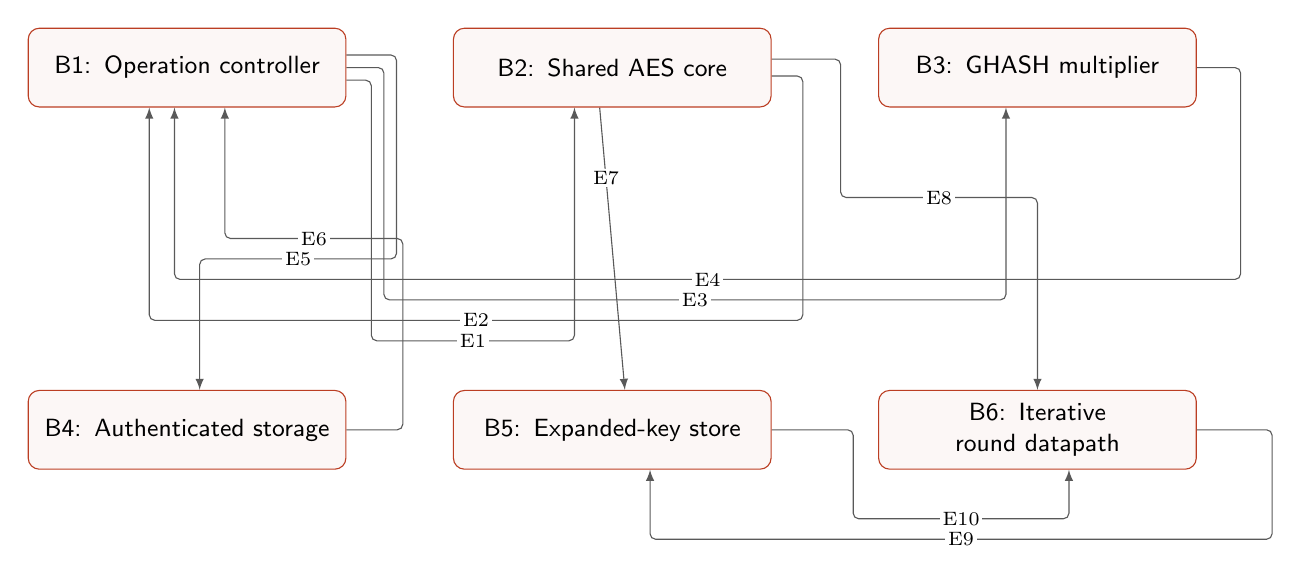
\begin{tikzpicture}[every node/.style={font=\small\sffamily},>=latex]

\node[draw=vulcan,rounded corners,fill=vulcan!4,text width=3.8cm,minimum height=1cm,align=center] (b0) at (0.0,0.0) {B1: Operation controller};

\node[draw=vulcan,rounded corners,fill=vulcan!4,text width=3.8cm,minimum height=1cm,align=center] (b1) at (5.4,0.0) {B2: Shared AES core};

\node[draw=vulcan,rounded corners,fill=vulcan!4,text width=3.8cm,minimum height=1cm,align=center] (b2) at (10.8,0.0) {B3: GHASH multiplier};

\node[draw=vulcan,rounded corners,fill=vulcan!4,text width=3.8cm,minimum height=1cm,align=center] (b3) at (0.0,-4.6) {B4: Authenticated storage};

\node[draw=vulcan,rounded corners,fill=vulcan!4,text width=3.8cm,minimum height=1cm,align=center] (b4) at (5.4,-4.6) {B5: Expanded-key store};

\node[draw=vulcan,rounded corners,fill=vulcan!4,text width=3.8cm,minimum height=1cm,align=center] (b5) at (10.8,-4.6) {B6: Iterative round datapath};

\begin{pgfonlayer}{connections}

\draw[->,black!65,rounded corners=2pt] ([yshift=-0.160cm]b0.east) -- (2.340,-0.160) -- (2.340,-3.470) -- coordinate[midway] (e0) (4.920,-3.470) -- ([xshift=-0.480cm]b1.south);

\draw[->,black!65,rounded corners=2pt] ([yshift=-0.107cm]b1.east) -- (7.820,-0.107) -- (7.820,-3.210) -- coordinate[midway] (e1) (-0.480,-3.210) -- ([xshift=-0.480cm]b0.south);

\draw[->,black!65,rounded corners=2pt] ([yshift=0.000cm]b0.east) -- (2.500,0.000) -- (2.500,-2.950) -- coordinate[midway] (e2) (10.400,-2.950) -- ([xshift=-0.400cm]b2.south);

\draw[->,black!65,rounded corners=2pt] ([yshift=0.000cm]b2.east) -- (13.380,0.000) -- (13.380,-2.690) -- coordinate[midway] (e3) (-0.160,-2.690) -- ([xshift=-0.160cm]b0.south);

\draw[->,black!65,rounded corners=2pt] ([yshift=0.160cm]b0.east) -- (2.660,0.160) -- (2.660,-2.430) -- coordinate[midway] (e4) (0.160,-2.430) -- ([xshift=0.160cm]b3.north);

\draw[->,black!65,rounded corners=2pt] ([yshift=0.000cm]b3.east) -- (2.740,-4.600) -- (2.740,-2.170) -- coordinate[midway] (e5) (0.480,-2.170) -- ([xshift=0.480cm]b0.south);

\draw[->,black!65] ([xshift=-0.160cm]b1.south) -- coordinate[pos=0.25] (e6) ([xshift=0.160cm]b4.north);

\draw[->,black!65,rounded corners=2pt] ([yshift=0.107cm]b1.east) -- (8.300,0.107) -- (8.300,-1.650) -- coordinate[midway] (e7) (10.800,-1.650) -- ([xshift=0.000cm]b5.north);

\draw[->,black!65,rounded corners=2pt] ([yshift=0.000cm]b5.east) -- (13.780,-4.600) -- (13.780,-5.990) -- coordinate[midway] (e8) (5.880,-5.990) -- ([xshift=0.480cm]b4.south);

\draw[->,black!65,rounded corners=2pt] ([yshift=0.000cm]b4.east) -- (8.460,-4.600) -- (8.460,-5.730) -- coordinate[midway] (e9) (11.200,-5.730) -- ([xshift=0.400cm]b5.south);

\end{pgfonlayer}

\begin{pgfonlayer}{edge labels}

\node[fill=white,inner sep=1pt,font=\scriptsize] at (e0) {E1};

\node[fill=white,inner sep=1pt,font=\scriptsize] at (e1) {E2};

\node[fill=white,inner sep=1pt,font=\scriptsize] at (e2) {E3};

\node[fill=white,inner sep=1pt,font=\scriptsize] at (e3) {E4};

\node[fill=white,inner sep=1pt,font=\scriptsize] at (e4) {E5};

\node[fill=white,inner sep=1pt,font=\scriptsize] at (e5) {E6};

\node[fill=white,inner sep=1pt,font=\scriptsize] at (e6) {E7};

\node[fill=white,inner sep=1pt,font=\scriptsize] at (e7) {E8};

\node[fill=white,inner sep=1pt,font=\scriptsize] at (e8) {E9};

\node[fill=white,inner sep=1pt,font=\scriptsize] at (e9) {E10};

\end{pgfonlayer}

\end{tikzpicture}\end{center}

{\small Functional block map, not a gate-level netlist. Edge identifiers match the directed relationships below. Crossings do not denote junctions; separate attachment points preserve arrow directions.}

{\small\begin{longtable}{@{}L{0.24\textwidth}L{0.7\textwidth}@{}}\toprule

\textbf{Block} & \textbf{Responsi\allowbreak{}bility}\\\midrule\endhead

B1: Operatio\allowbreak{}n controll\allowbreak{}er & rivet\_\allowbreak{}a2\_\allowbreak{}top owns arbitrat\allowbreak{}ion,\allowbreak{} command capture,\allowbreak{} counter formatio\allowbreak{}n,\allowbreak{} byte masking,\allowbreak{} stream ordering,\allowbreak{} tag comparis\allowbreak{}on,\allowbreak{} scrubbin\allowbreak{}g and output selectio\allowbreak{}n.\\[3pt]

B2: Shared AES core & u\_\allowbreak{}aes\_\allowbreak{}core coordina\allowbreak{}tes key expansio\allowbreak{}n and iterativ\allowbreak{}e block processi\allowbreak{}ng for raw AES,\allowbreak{} GCM hash-subkey derivati\allowbreak{}on,\allowbreak{} tag masking and payload keystrea\allowbreak{}m generati\allowbreak{}on.\\[3pt]

B3: GHASH multipli\allowbreak{}er & u\_\allowbreak{}ghash performs one GF(\allowbreak{}2\textasciicircum{}128)\allowbreak{} multipli\allowbreak{}cation in 128 processi\allowbreak{}ng clocks,\allowbreak{} with explicit start,\allowbreak{} busy,\allowbreak{} done and clear controls.\\[3pt]

B4: Authenti\allowbreak{}cated storage & Controll\allowbreak{}er-owned payload\_\allowbreak{}store and byte\_\allowbreak{}store retain 128 data bits and five length bits per entry. Failed operatio\allowbreak{}ns scrub every entry before presenti\allowbreak{}ng tag status.\\[3pt]

B5: Expanded-key store & u\_\allowbreak{}key\_\allowbreak{}schedule stores 60 words of 32 bits; AES-128 uses 44 words. Expansio\allowbreak{}n computes one new word per clock and supplies selected round keys.\\[3pt]

B6: Iterativ\allowbreak{}e round datapath & u\_\allowbreak{}datapath performs initial AddRound\allowbreak{}Key and one round per clock. Connecte\allowbreak{}d u\_\allowbreak{}sbox,\allowbreak{} u\_\allowbreak{}shiftrow\allowbreak{}s and u\_\allowbreak{}mixcolum\allowbreak{}ns implemen\allowbreak{}t real forward and inverse transfor\allowbreak{}mations.\\[3pt]

\bottomrule\end{longtable}}

{\small\begin{longtable}{@{}L{0.24\textwidth}L{0.7\textwidth}@{}}\toprule

\textbf{Directed relation\allowbreak{}ship} & \textbf{Meaning}\\\midrule\endhead

E1: B1 to B2 & Key loads and AES block requests\\[3pt]

E2: B2 to B1 & AES results and service readines\allowbreak{}s\\[3pt]

E3: B1 to B3 & Hash operands,\allowbreak{} subkey and service control\\[3pt]

E4: B3 to B1 & Complete\allowbreak{}d authenti\allowbreak{}cation products\\[3pt]

E5: B1 to B4 & Payload writes,\allowbreak{} drain ownershi\allowbreak{}p and erasure\\[3pt]

E6: B4 to B1 & Buffered payload and byte counts\\[3pt]

E7: B2 to B5 & Accepted key and length selectio\allowbreak{}n\\[3pt]

E8: B2 to B6 & Block request and output handshak\allowbreak{}e\\[3pt]

E9: B6 to B5 & Round-key index\\[3pt]

E10: B5 to B6 & Selected round key and round count\\[3pt]

\bottomrule\end{longtable}}

\section{Interfaces and configuration}

{\small\begin{longtable}{@{}L{0.2\textwidth}L{0.12\textwidth}L{0.1\textwidth}L{0.48\textwidth}@{}}\toprule

\textbf{Signal /\allowbreak{} group} & \textbf{Directio\allowbreak{}n} & \textbf{Width} & \textbf{Contract}\\\midrule\endhead

clk,\allowbreak{} rst\_\allowbreak{}n & Input & 1 bit each & Rising-edge clock and asynchro\allowbreak{}nous active-low reset. Reset aborts work,\allowbreak{} clears keys and storage,\allowbreak{} and forces every public output to zero.\\[3pt]

key\_\allowbreak{}valid,\allowbreak{} key\_\allowbreak{}in,\allowbreak{} key\_\allowbreak{}len\_\allowbreak{}sel & Input & 1,\allowbreak{} 256,\allowbreak{} 1 bits & Capture on key\_\allowbreak{}valid \&\& key\_\allowbreak{}ready. Selectio\allowbreak{}n 0 uses key\_\allowbreak{}in[\allowbreak{}255:128]\allowbreak{} for AES-128 and ignores the lower half; selectio\allowbreak{}n 1 uses all 256 bits.\\[3pt]

key\_\allowbreak{}ready,\allowbreak{} key\_\allowbreak{}loaded & Output & 1 bit each & Indicate key-load acceptan\allowbreak{}ce readines\allowbreak{}s and complete\allowbreak{}d expansio\allowbreak{}n. Loading is restrict\allowbreak{}ed to idle with no outstand\allowbreak{}ing tag or payload.\\[3pt]

in\_\allowbreak{}valid,\allowbreak{} in\_\allowbreak{}enc\_\allowbreak{}dec,\allowbreak{} in\_\allowbreak{}block,\allowbreak{} in\_\allowbreak{}tag\_\allowbreak{}id & Input & 1,\allowbreak{} 1,\allowbreak{} 128,\allowbreak{} 8 bits & Raw AES request captured on in\_\allowbreak{}valid \&\& in\_\allowbreak{}ready. Directio\allowbreak{}n 0 encrypts and 1 decrypts; the identifi\allowbreak{}er accompan\allowbreak{}ies the result.\\[3pt]

in\_\allowbreak{}ready,\allowbreak{} cmd\_\allowbreak{}ready,\allowbreak{} data\_\allowbreak{}ready & Output & 1 bit each & Acceptan\allowbreak{}ce readines\allowbreak{}s for raw requests,\allowbreak{} GCM commands and stream beats respecti\allowbreak{}vely. Traffic without its correspo\allowbreak{}nding handshak\allowbreak{}e has no effect.\\[3pt]

cmd\_\allowbreak{}valid,\allowbreak{} cmd\_\allowbreak{}decrypt,\allowbreak{} iv\_\allowbreak{}in & Input & 1,\allowbreak{} 1,\allowbreak{} 96 bits & GCM request,\allowbreak{} directio\allowbreak{}n and IV,\allowbreak{} captured on cmd\_\allowbreak{}valid \&\& cmd\_\allowbreak{}ready. cmd\_\allowbreak{}decrypt=\allowbreak{}1 selects authenti\allowbreak{}cated decrypti\allowbreak{}on.\\[3pt]

aad\_\allowbreak{}bytes,\allowbreak{} payload\_\allowbreak{}bytes,\allowbreak{} expected\_\allowbreak{}tag & Input & 32,\allowbreak{} 32,\allowbreak{} 128 bits & Unsigned section lengths in bytes and the full expected decrypti\allowbreak{}on tag; captured with the GCM command.\\[3pt]

data\_\allowbreak{}valid,\allowbreak{} data\_\allowbreak{}is\_\allowbreak{}aad,\allowbreak{} data\_\allowbreak{}in,\allowbreak{} valid\_\allowbreak{}bytes & Input & 1,\allowbreak{} 1,\allowbreak{} 128,\allowbreak{} 5 bits & Stream record captured on data\_\allowbreak{}valid \&\& data\_\allowbreak{}ready. Section 1 denotes AAD and 0 payload. The first byte occupies bits [\allowbreak{}127:120]\allowbreak{}.\\[3pt]

out\_\allowbreak{}ready,\allowbreak{} tag\_\allowbreak{}ready & Input & 1 bit each & Independ\allowbreak{}ent consumpt\allowbreak{}ion controls for payload and tag/\allowbreak{}status records.\\[3pt]

out\_\allowbreak{}valid,\allowbreak{} out\_\allowbreak{}block,\allowbreak{} out\_\allowbreak{}tag\_\allowbreak{}id,\allowbreak{} out\_\allowbreak{}enc\_\allowbreak{}dec & Output & 1,\allowbreak{} 128,\allowbreak{} 8,\allowbreak{} 1 bits & Shared raw/\allowbreak{}GCM payload record. Stable while stalled; data and metadata are zero whenever out\_\allowbreak{}valid=\allowbreak{}0.\\[3pt]

out\_\allowbreak{}valid\_\allowbreak{}bytes,\allowbreak{} out\_\allowbreak{}is\_\allowbreak{}gcm & Output & 5,\allowbreak{} 1 bits & Exact payload length and mode discrimi\allowbreak{}nator. Raw results use 16 bytes and discrimi\allowbreak{}nator 0. GCM uses discrimi\allowbreak{}nator 1 and identifi\allowbreak{}er zero.\\[3pt]

tag\_\allowbreak{}valid,\allowbreak{} tag\_\allowbreak{}out,\allowbreak{} tag\_\allowbreak{}match,\allowbreak{} auth\_\allowbreak{}fail,\allowbreak{} protocol\_\allowbreak{}error & Output & 1,\allowbreak{} 128,\allowbreak{} 1,\allowbreak{} 1,\allowbreak{} 1 bits & One tag/\allowbreak{}status record per complete\allowbreak{}d,\allowbreak{} non-reset-aborted command. The entire record remains stable under tag backpres\allowbreak{}sure. Status persists after consumpt\allowbreak{}ion until the next accepted operatio\allowbreak{}n; tag\_\allowbreak{}out clears when tag\_\allowbreak{}valid clears.\\[3pt]

busy,\allowbreak{} err\_\allowbreak{}unloaded\_\allowbreak{}key & Output & 1 bit each & busy includes expansio\allowbreak{}n,\allowbreak{} processi\allowbreak{}ng,\allowbreak{} scrubbin\allowbreak{}g,\allowbreak{} tag wait and payload drain. err\_\allowbreak{}unloaded\_\allowbreak{}key is always zero: unloaded-key requests are backpres\allowbreak{}sured rather than accepted as errors.\\[3pt]

\bottomrule\end{longtable}}

{\small\begin{longtable}{@{}L{0.23\textwidth}L{0.12\textwidth}L{0.57\textwidth}@{}}\toprule

\textbf{Paramete\allowbreak{}r} & \textbf{Default} & \textbf{Meaning /\allowbreak{} supporte\allowbreak{}d values}\\\midrule\endhead

MAX\_\allowbreak{}PAYLOAD\_\allowbreak{}BLOCKS & 16 & Integer values 1 through 256 are supporte\allowbreak{}d. Both GCM directio\allowbreak{}ns accept at most 16*\allowbreak{}MAX\_\allowbreak{}PAYLOAD\_\allowbreak{}BLOCKS payload bytes: 256 bytes by default and 4096 bytes maximum. AAD is streamed independ\allowbreak{}ently of payload capacity. Unsuppor\allowbreak{}ted values are outside the contract and are not silently clamped.\\[3pt]

\bottomrule\end{longtable}}

\section{Behavior and corner cases}

\subsection{Admission and key lifetime}

Idle priority is key load,\allowbreak{} then GCM command,\allowbreak{} then raw block; readiness prevents simultaneous acceptance. Raw and GCM requests require a fully expanded key. Key material persists between operations until reset or accepted replacement. No new operation is accepted at the edge consuming the last result or tag.

\subsection{AES numerical and cycle semantics}

AES uses FIPS 197 column-major byte mapping,\allowbreak{} initial AddRoundKey,\allowbreak{} 10 rounds for AES-128 or 14 for AES-256,\allowbreak{} and no final MixColumns. AES-256 includes the additional SubWord at word index modulo eight equal to four. Raw decryption uses ordinary inverse AES. For acceptance at edge E,\allowbreak{} the completed raw result appears post-E+\allowbreak{}10 or post-E+\allowbreak{}14. Expansion completes post-E+\allowbreak{}40 or post-E+\allowbreak{}52 for a key accepted at E; top-level operation readiness resumes after controller retirement.

\subsection{GCM arithmetic}

Each command derives H=\allowbreak{}E\_\allowbreak{}K(\allowbreak{}0\textasciicircum{}128)\allowbreak{} and the tag mask E\_\allowbreak{}K(\allowbreak{}J0)\allowbreak{},\allowbreak{} where J0=\allowbreak{}IV||32'h00000001. Payload keystream starts at IV||32'h00000002 and increments only the low 32 counter bits. Both directions use forward AES. GHASH processes padded AAD,\allowbreak{} padded ciphertext and the length block [\allowbreak{}len(\allowbreak{}A)\allowbreak{}]\allowbreak{}64||[\allowbreak{}len(\allowbreak{}C)\allowbreak{}]\allowbreak{}64 in bits. Byte counts are widened to 64 bits before multiplication by eight. The field polynomial is x\textasciicircum{}128+\allowbreak{}x\textasciicircum{}7+\allowbreak{}x\textasciicircum{}2+\allowbreak{}x+\allowbreak{}1; the RTL uses MSB-first processing,\allowbreak{} right shifts and reduction constant 128'he1000000000000000000000000000000. The tag is E\_\allowbreak{}K(\allowbreak{}J0)\allowbreak{} XOR final GHASH.

\subsection{Stream boundaries and masking}

Exactly aad\_\allowbreak{}bytes of AAD precede exactly payload\_\allowbreak{}bytes of payload; empty sections consume no beats. Each accepted beat must contain min(\allowbreak{}16,\allowbreak{} remaining section bytes)\allowbreak{},\allowbreak{} from 1 through 16. Unused low-order bytes are ignored and zero-padded before hashing. Partial payload outputs also have zero unused bytes. Encryption hashes generated ciphertext; decryption hashes received ciphertext.

\subsection{Authentication and erasure}

All 128 expected-tag bits participate in one equality decision without mismatch-position early exit. Encryption reports tag\_\allowbreak{}match=\allowbreak{}0 and auth\_\allowbreak{}fail=\allowbreak{}0; successful decryption reports 1 and 0; failed decryption reports 0 and 1. Failure scrubs one storage entry per clock across the configured capacity,\allowbreak{} independently of either output-ready signal,\allowbreak{} before tag\_\allowbreak{}valid. The calculated tag is returned on authentication failure,\allowbreak{} but no payload is released. Successful payload entries are erased as consumed,\allowbreak{} and transient payload registers clear when no longer needed.

\subsection{Public handshake timeline}

Transfers use pre-edge valid \&\& ready; newly created records are visible post-edge and cannot transfer at their creation edge. The first rising edge after reset release enables readiness but accepts nothing. Following command acceptance,\allowbreak{} H and tag-mask derivation precede data readiness. Accepted beats temporarily close data readiness while processed. After final length hashing,\allowbreak{} a successful tag is presented,\allowbreak{} or scrubbing precedes a failure/\allowbreak{}error tag. If that tag transfers at U,\allowbreak{} successful nonempty payload first appears post-U and cannot transfer before U+\allowbreak{}1. The last payload transfer returns idle post-edge. Empty successes and failures return idle after tag consumption.

\subsection{Malformed transactions and recovery}

An oversized command is accepted as an error without consuming stream data. An accepted wrong section indicator or byte count aborts processing. Both paths scrub storage and emit one record with tag\_\allowbreak{}out=\allowbreak{}0,\allowbreak{} protocol\_\allowbreak{}error=\allowbreak{}1,\allowbreak{} tag\_\allowbreak{}match=\allowbreak{}0 and auth\_\allowbreak{}fail=\allowbreak{}0,\allowbreak{} with no payload output. After status consumption,\allowbreak{} a new transaction may begin. Reset overrides every phase and clears outstanding state.

\section{Verification methods and measured results}

\subsection{Independent cryptographic reference}

\textbf{Method.} Standard-library Python computes AES substitution algebraically and GHASH through polynomial convolution and long division. Published anchors are checked before generating RTL expectations: FIPS 197 Appendix C.1/\allowbreak{}C.3 and McGrew/\allowbreak{}Viega GCM submission Appendix B cases 1,\allowbreak{} 2,\allowbreak{} 4,\allowbreak{} 13,\allowbreak{} 14 and 16.

\textbf{Result.} Two AES anchors,\allowbreak{} including inverse checks,\allowbreak{} and six GCM anchors passed. GCM anchors cover empty,\allowbreak{} single-block and 60-byte payload/\allowbreak{}20-byte AAD partial-final messages for both key sizes. Exact vector provenance is retained in reference\_\allowbreak{}anchors.json.

{\small Evidence: E018,\allowbreak{} E028}

\subsection{Internal service contracts}

\textbf{Method.} Standalone port-level tests compare expanded keys and independent field products,\allowbreak{} including service timing,\allowbreak{} busy-start rejection and clear behavior.

\textbf{Result.} 37 round-key comparisons across AES-128/\allowbreak{}256/\allowbreak{}128 rekeys and 16 GHASH product comparisons passed; expansion completed at 40/\allowbreak{}52 edges and multiplication at 128 edges.

{\small Evidence: E020,\allowbreak{} E028}

\subsection{Capacity-one behavior}

\textbf{Method.} Seed 1701 public-interface simulation; exact payload,\allowbreak{} tags,\allowbreak{} metadata,\allowbreak{} lengths and transfer counts.

\textbf{Result.} Passed 78,\allowbreak{}813 observed cycles,\allowbreak{} 68 raw results,\allowbreak{} 142 tag records and 110 GCM payload records; 18 intentional protocol-error records were checked.

{\small Evidence: E028}

\subsection{Non-power-of-two capacity}

\textbf{Method.} The same checker at capacity 3,\allowbreak{} seed 1701.

\textbf{Result.} Passed 91,\allowbreak{}263 observed cycles,\allowbreak{} 68 raw results,\allowbreak{} 144 tag records and 190 GCM payload records; 20 intentional protocol-error records were checked.

{\small Evidence: E028}

\subsection{Default-capacity functional and adversarial coverage}

\textbf{Method.} Capacity 16,\allowbreak{} seed 1701,\allowbreak{} including 20 additional differential message shapes per key size,\allowbreak{} every expected-tag bit corrupted separately for each key size,\allowbreak{} and independent AAD,\allowbreak{} IV and ciphertext mutations.

\textbf{Result.} Passed 387,\allowbreak{}904 observed cycles,\allowbreak{} 68 raw results,\allowbreak{} 450 tag records and 683 GCM payload records. All 256 single-bit tag-corruption cases were rejected with equal failure latency for otherwise identical timing within each key size.

{\small Evidence: E019,\allowbreak{} E028}

\subsection{Maximum supported payload}

\textbf{Method.} Capacity 256 elaboration and simulation,\allowbreak{} seed 1701,\allowbreak{} including full 4096-byte encryption and decryption for both key sizes.

\textbf{Result.} Passed 163,\allowbreak{}543 observed cycles,\allowbreak{} 26 tag records and 1,\allowbreak{}026 payload records. Maximum-capacity functional coverage is distinct from the smaller-capacity synthesis matrix.

{\small Evidence: E028}

\subsection{Release protection,\allowbreak{} reset and protocol boundaries}

\textbf{Method.} Continuous public-output assertions,\allowbreak{} input gaps,\allowbreak{} output/\allowbreak{}tag stalls,\allowbreak{} arbitration,\allowbreak{} reset during expansion/\allowbreak{}processing/\allowbreak{}stalls,\allowbreak{} malformed traffic and checked recovery. Capacities 1,\allowbreak{} 3 and 16 exercise every final byte count 1 through 16 for both key sizes and directions.

\textbf{Result.} No checked pre-authentication or failed-message payload release,\allowbreak{} active-output X/\allowbreak{}Z,\allowbreak{} stalled-record instability or inactive-data leakage occurred. Exact-capacity acceptance and capacity-plus-one rejection passed.

{\small Evidence: E012,\allowbreak{} E016,\allowbreak{} E028}

\subsection{Checker sensitivity}

\textbf{Method.} The same real checker tests a passing capacity-3 baseline and six independent disposable RTL mutations; production RTL is unchanged.

\textbf{Result.} Six of six mutants were functionally rejected: missing AES-256 extra SubWord produced an AES mismatch; incorrect GHASH reduction,\allowbreak{} masking,\allowbreak{} length formation and tag comparison produced tag/\allowbreak{}status mismatches; premature plaintext visibility triggered the release assertion. Compilation failures were not counted.

{\small Evidence: E021,\allowbreak{} E029}

\subsection{Generic synthesizability and structure}

\textbf{Method.} Yosys read/\allowbreak{}elaborate,\allowbreak{} explicit top selection,\allowbreak{} hierarchy and consistency checks,\allowbreak{} generic synthesis and retained netlists at capacities 1,\allowbreak{} 3 and 16.

\textbf{Result.} All three passed with zero latches and unresolved modules,\allowbreak{} all seven required literal instances,\allowbreak{} and no accepted driver-conflict or combinational-loop diagnostics. Payload storage was 133/\allowbreak{}399/\allowbreak{}2,\allowbreak{}128 bits; post-synthesis sequential state was 4,\allowbreak{}163/\allowbreak{}4,\allowbreak{}429/\allowbreak{}6,\allowbreak{}158 bits respectively.

{\small Evidence: E021,\allowbreak{} E030}

\subsection{Stable verification inputs}

\textbf{Method.} Repair startup bytecode generation that changed files covered by the verification input selector; retain the original rejected execution and rerun the admitted behavior check.

\textbf{Result.} Disabling bytecode writes before local imports resolved the input-stability failure without changing RTL or acceptance criteria. The rejected execution is excluded from the functional ledger above.

{\small Evidence: E017,\allowbreak{} E021,\allowbreak{} E026,\allowbreak{} E027,\allowbreak{} E028}

\section{Integration and use}

Instantiate rivet\_\allowbreak{}a2\_\allowbreak{}top from \texttt{rtl/\allowbreak{}rivet\_\allowbreak{}a2\_\allowbreak{}top.sv}. Compile \texttt{rtl/\allowbreak{}rivet\_\allowbreak{}a2\_\allowbreak{}pkg.sv} first,\allowbreak{} followed by the other \texttt{rtl/\allowbreak{}*\allowbreak{}.sv} files. The 256-bit key port requires explicit adaptation from Gen-1 integrations; functional continuity does not imply pin compatibility.


Assert rst\_\allowbreak{}n low,\allowbreak{} release reset,\allowbreak{} and wait for key\_\allowbreak{}ready before transferring a key. Wait for operation readiness rather than assuming key\_\allowbreak{}loaded alone admits a request. Preserve each request until its handshake.


For GCM,\allowbreak{} supply a unique encryption IV under each key,\allowbreak{} transfer the command,\allowbreak{} then stream the declared AAD and payload with the required section and byte-count fields. Consume and inspect tag status before accepting the subsequent payload stream.


Use installed python3,\allowbreak{} iverilog,\allowbreak{} vvp and yosys. Observed versions were Python 3.12.3,\allowbreak{} Icarus/\allowbreak{}vvp 12.0 and Yosys 0.33. From the project root run \texttt{python3 tests/\allowbreak{}verify.py --check behavior},\allowbreak{} \texttt{python3 tests/\allowbreak{}verify.py --check sensitivity} and \texttt{python3 tests/\allowbreak{}verify.py --check synthesis}.


Each check creates fresh outputs under \texttt{evidence/\allowbreak{}checks/\allowbreak{}verifier-<check>-<UTC>-<id>/\allowbreak{}}. Its \texttt{results.json} links source hashes,\allowbreak{} snapshots,\allowbreak{} comparison counts,\allowbreak{} command receipts and raw evidence. \texttt{tests/\allowbreak{}README.md} supplies the executable requirement map and evidence-navigation contract. Earlier design-document placeholders do not supersede these completed results.


Yosys 0.33 requires the verifier's mechanical package-import expansion. Generated synthesis inputs and \texttt{frontend-mapping.json} preserve the original-to-generated relationship; Icarus tests the original package-form RTL. Designer-owned RTL/\allowbreak{}documentation and independently authored tests remain separate delivery sources.


\section{Limitations and acceptance boundary}

Only 96-bit IVs and full 128-bit tags are supported. Nonce uniqueness is an application responsibility; persistent reuse detection is not implemented.


Payload capacity is finite and applies to both directions. AAD has a 32-bit byte-count interface,\allowbreak{} but exhaustive testing of that entire range is not claimed.


One operation is active at a time. GCM latency depends on message size,\allowbreak{} serialized AES/\allowbreak{}GHASH work and external handshakes; no clock-frequency or throughput target was measured.


Simulation covers a deterministic bounded matrix,\allowbreak{} not exhaustive state exploration or formal proof. Synthesis covers capacities 1,\allowbreak{} 3 and 16,\allowbreak{} not every supported value or capacity 256.


Logical scrubbing and constant mismatch-position comparison behavior do not establish physical side-channel resistance,\allowbreak{} fault resistance or power-remanence erasure. Keys are intentionally retained between operations.


No process mapping,\allowbreak{} physical area,\allowbreak{} power,\allowbreak{} timing closure,\allowbreak{} FPGA demonstration or tapeout readiness is established. Generic sequential-bit counts are structural measurements,\allowbreak{} not silicon area.


The documented checks were executed in the project workspace. A separate clean-directory portable-delivery reproduction was not established.


\appendix\section{Source inventory}

Production inventory: 9 Verilog/\allowbreak{}SystemVerilog files; 892 nonblank,\allowbreak{} non-comment lines. Source size is not a correctness or quality metric.

{\small\begin{longtable}{@{}L{0.61\textwidth}L{0.15\textwidth}L{0.15\textwidth}@{}}\toprule

\textbf{Producti\allowbreak{}on file} & \textbf{Physical lines} & \textbf{Code lines}\\\midrule\endhead

rtl/\allowbreak{}rivet\_\allowbreak{}a2\_\allowbreak{}aes\_\allowbreak{}core.sv & 47 & 45\\[3pt]

rtl/\allowbreak{}rivet\_\allowbreak{}a2\_\allowbreak{}datapath.sv & 85 & 81\\[3pt]

rtl/\allowbreak{}rivet\_\allowbreak{}a2\_\allowbreak{}ghash.sv & 62 & 61\\[3pt]

rtl/\allowbreak{}rivet\_\allowbreak{}a2\_\allowbreak{}key\_\allowbreak{}schedule.sv & 89 & 86\\[3pt]

rtl/\allowbreak{}rivet\_\allowbreak{}a2\_\allowbreak{}mixcolum\allowbreak{}ns.sv & 23 & 23\\[3pt]

rtl/\allowbreak{}rivet\_\allowbreak{}a2\_\allowbreak{}pkg.sv & 104 & 97\\[3pt]

rtl/\allowbreak{}rivet\_\allowbreak{}a2\_\allowbreak{}sbox.sv & 14 & 14\\[3pt]

rtl/\allowbreak{}rivet\_\allowbreak{}a2\_\allowbreak{}shiftrow\allowbreak{}s.sv & 16 & 16\\[3pt]

rtl/\allowbreak{}rivet\_\allowbreak{}a2\_\allowbreak{}top.sv & 474 & 469\\[3pt]

\bottomrule\end{longtable}}

\section{Verification record index}

{\small\begin{longtable}{@{}L{0.57\textwidth}L{0.16\textwidth}L{0.17\textwidth}@{}}\toprule

\textbf{Recorded check} & \textbf{Outcome} & \textbf{Executio\allowbreak{}n time (\allowbreak{}s)\allowbreak{}}\\\midrule\endhead

behavior & passed & 162.649\\[3pt]

sensitiv\allowbreak{}ity & passed & 7.231\\[3pt]

synthesi\allowbreak{}s & passed & 383.297\\[3pt]

\bottomrule\end{longtable}}

Execution times include tool and provider waiting; they are not hardware latency or model utilization.

{\small\begin{longtable}{@{}L{0.12\textwidth}L{0.82\textwidth}@{}}\toprule

\textbf{Referenc\allowbreak{}e} & \textbf{Original project-relative record}\\\midrule\endhead

E012 & tests/\allowbreak{}README.md\\[3pt]

E016 & tests/\allowbreak{}bridge.sv\\[3pt]

E017 & tests/\allowbreak{}input\_\allowbreak{}stabilit\allowbreak{}y.py\\[3pt]

E018 & tests/\allowbreak{}referenc\allowbreak{}e.py\\[3pt]

E019 & tests/\allowbreak{}scenario\allowbreak{}s.py\\[3pt]

E020 & tests/\allowbreak{}units.py\\[3pt]

E021 & tests/\allowbreak{}verify.py\\[3pt]

E026 & .vulcan/\allowbreak{}engineer\allowbreak{}ing/\allowbreak{}run-0001/\allowbreak{}attempt-0003/\allowbreak{}stdout.log\\[3pt]

E027 & .vulcan/\allowbreak{}engineer\allowbreak{}ing/\allowbreak{}run-0001/\allowbreak{}attempt-0004/\allowbreak{}response.json\\[3pt]

E028 & .vulcan/\allowbreak{}engineer\allowbreak{}ing/\allowbreak{}run-0001/\allowbreak{}attempt-0005/\allowbreak{}stdout.log\\[3pt]

E029 & .vulcan/\allowbreak{}engineer\allowbreak{}ing/\allowbreak{}run-0001/\allowbreak{}attempt-0006/\allowbreak{}stdout.log\\[3pt]

E030 & .vulcan/\allowbreak{}engineer\allowbreak{}ing/\allowbreak{}run-0001/\allowbreak{}attempt-0007/\allowbreak{}stdout.log\\[3pt]

\bottomrule\end{longtable}}

\section{Document provenance}

Engineering was independently accepted for the recorded source and evidence identity. This is not exhaustive proof, hardware deployment or physical signoff. The companion REPORT.md records the exact report approval and source manifest, and links the English/Chinese journeys containing original failures and interventions. A report number identifies a generation attempt, not a new hardware revision.

No developer attribution was supplied; none has been inferred.

\end{document}
